% 
% Annual Cognitive Science Conference
% Sample LaTeX Paper -- Proceedings Format
% 

% Original : Ashwin Ram (ashwin@cc.gatech.edu)       04/01/1994
% Modified : Johanna Moore (jmoore@cs.pitt.edu)      03/17/1995
% Modified : David Noelle (noelle@ucsd.edu)          03/15/1996
% Modified : Pat Langley (langley@cs.stanford.edu)   01/26/1997
% Latex2e corrections by Ramin Charles Nakisa        01/28/1997 
% Modified : Tina Eliassi-Rad (eliassi@cs.wisc.edu)  01/31/1998
% Modified : Trisha Yannuzzi (trisha@ircs.upenn.edu) 12/28/1999 (in process)
% Modified : Mary Ellen Foster (M.E.Foster@ed.ac.uk) 12/11/2000
% Modified : Ken Forbus                              01/23/2004
% Modified : Eli M. Silk (esilk@pitt.edu)            05/24/2005
% Modified: Niels Taatgen (taatgen@cmu.edu) 10/24/2006

%% Change ``a4paper'' in the following line to ``letterpaper'' if you are
%% producing a letter-format document.

\documentclass[10pt,letterpaper]{article}
\usepackage{url}
\usepackage{graphicx}
\usepackage{cogsci}
\usepackage{pslatex}
\usepackage{apacite}
\usepackage{amssymb,amsfonts,amsmath}
\usepackage{booktabs, colortbl, tabularx}
\usepackage[table]{xcolor}

\title{Formalizing the Pragmatics of Metaphor Understanding}
 

  \author{{\large {\bf Justine T. Kao$^1$} (justinek@stanford.edu)}, {\large {\bf Leon Bergen$^2$} (bergen@mit.edu)}, {\large {\bf Noah D.~Goodman$^1$} (ngoodman@stanford.edu)}\\
  $^1$Department of Psychology, Stanford University. $^2$Department of Brain and Cognitive Science, MIT. }
 

\begin{document}

\maketitle
\begin{abstract}
While the ubiquity and importance of nonliteral language are clear, people's ability to use and understand it remains a mystery. Metaphor in particular has been studied extensively across many disciplines in cognitive science. One approach focuses on the pragmatic principles that listeners utilize to infer meaning from metaphorical utterances. While this approach has generated a number of insights about how people understand metaphor, to our knowledge there is no formal model showing that effects in metaphor understanding can arise from basic principles of communication. Building upon recent advances in formal models of pragmatics, we describe a computational model that uses pragmatic reasoning to interpret metaphorical utterances. We conduct behavioral experiments to evaluate the model's performance and show that our model produces metaphorical interpretations that closely fit behavioral data. We discuss implications of the model for metaphor understanding, principles of communication, and formal models of language understanding.

\textbf{Keywords:} 
language understanding; metaphor; pragmatics; computational models
\end{abstract}


\section{Introduction}
From ``Juliet is the sun" to ``That woman is a bombshell," nonliteral language is, quite literally, everywhere. Metaphor, hyperbole, and sarcasm are ubiquitous features of human communication, often creating poetic or humorous effects that add rich dimensions to language \cite{glucksberg2001understanding, pilkington2000poetic, lakoff2009more, roberts1994people}. Metaphor has inspired a particularly large amount of research in cognitive science, spanning topics such as how metaphors structure and shape our thoughts \cite{ortony1993metaphor, lakoff1993contemporary, thibodeau2011metaphors}, whether metaphor processing recruits the same strategies as standard language processing \cite{giora1997understanding, gibbs2002new, glucksberg1993metaphors} and what factors determine the meaning and aptness of a novel metaphor \cite{blasko1993effects, tourangeau1981aptness, kintsch2002metaphor}. This overwhelming interest in metaphor research is due to both the ubiquity of metaphor in everyday language and the potential role of metaphor for helping us understand how the mind creates meaning. 

One approach to studying metaphor focuses on the pragmatic principles that listeners utilize to infer meaning from metaphorical utterances \cite{tendahl2008complementary}. Rather than view metaphor as a separate mode of communication that requires specialized language processing strategies, this approach argues that basic principles of communication drive the meaning that a listener infers from a metaphor \cite{sperber2008deflationary, wilson2006metaphor}. Relevance theory, in particular, posits that listeners interpret utterances with the assumption that speakers produced them because they are maximally relevant \cite{wilson2002relevance}. Relevance theorists argue that this principle explains how listeners infer the meaning of a novel metaphor as well as other forms of loose talk where the meaning of an utterance is underspecified  \cite{sperber1985loose}. When interpreting the metaphor ``My lawyer is a shark," for example, the listener assumes that the speaker aims to communicate features of  ``a shark" that are relevant to the person under discussion (``my lawyer") and do not make use of other shark features---\emph{vicious} but not \emph{has fins} or \emph{swims}.

While many linguists and psychologists have argued for the benefits of studying metaphor using a pragmatics framework, to our knowledge there is no formal model showing that effects in metaphor understanding may arise from basic principles of communication. On the other hand, a recent body of work presents a series of computational models for pragmatic reasoning, where speaker and listener reason about each other to communicate effectively \cite{frank2012predicting, jager2009pragmatic}. By formalizing principles of communication, these models are able to make quantitative predictions about a range of phenomena in language understanding, such as scalar implicature and the effect of alternative utterances \cite{goodman2013knowledge, bergen2012s}. However, a limitation of these models is that they are unable to explain the use of utterances which are known to have false literal interpretations. More recent work extends these models to consider affective goals in communication that may be optimally satisfied by nonliteral utterances such as hyperbole (under review). In this paper, we will be considering the role of communicative goals in the interpretation of metaphorical utterances. In our formalization, a listener assumes that the speaker chooses an utterance to maximize informativeness about a subject along dimensions that are relevant to the conversation and consistent with the speaker's communicative goal. This makes it possible for a literally false utterance to be optimal as long as it is informative along the target dimension. Our framework closely aligns with the relevance-theoretic view that a listener considers the relevance of a potential meaning to the speaker's goal in order to infer what the speaker intended to communicate. 

%Although metaphor understanding is a complex phenomenon that calls for a variety of approaches, we present a computational model to argue that the interpretation of at least some types of metaphor are shaped by principles of pragmatics. 
To reasonably limit the scope of our work, we focus on metaphors of the classic form ``$X$ is a $Y$." We describe a computational model that can interpret such sentences metaphorically and conduct behavioral experiments to evaluate the model's performance. We show that peoples' interpretations of metaphors are driven by conversational context and that our model captures this effect. Finally, we show that our model predictions correlate significantly with people's fine-grained interpretations of metaphorical utterances.

\section{Computational Model}
In the basic Rational Speech Act model of \cite{frank2012predicting, goodman2013knowledge}, a listener and a speaker recursively reason about each other to arrive at pragmatically enriched meanings. Given an intended meaning, a speaker reasons about a literal listener and chooses an utterance based on its informativeness. A pragmatic listener then reasons about the speaker and uses Bayes' rule to infer the meaning given the utterance. To account for nonliteral interpretation, we extend this model by considering the idea that a speaker may have a range of different communicative goals. Intuitively, an utterance is optimally informative and relevant if it satisfies the speaker's communicative goal. Since the speaker's precise communicative goal may be unknown to the listener, the listener performs joint inference on the goal as well as the intended meaning. By introducing multiple potential goals for communication, we open up the possibility for a speaker to produce an utterance that is literally false but still satisfies her goal. The speaker achieves this in part by exploiting her own and the listener's prior knowledge---their common ground \cite{clark1996using}---to reason about what information the listener would gain if he takes the utterance literally. 

To illustrate this idea more concretely and demonstrate how it is implemented in our model, we will use the metaphor ``John is a shark" as an example. For simplicity, in this model we restrict the number of possible categories to which a member may belong to $c_a$ and $c_p$, denoting an animal category or a person category, respectively. We also restrict the possible features of John under consideration to a vector of size three: $\vec f = [f_1, f_2, f_3]$, where $f_i$ is either $0$ or $1$ (for example, the three features could be scary, sleek, and finned).
The literal listener $L_0$ will interpret the utterance ``John is a shark" as meaning that John is literally a member of the category ``shark" and has corresponding features. Formally, if $u$ is the uttered category:
\[ L_0(c, \vec f |u) = \left\{ 
  \begin{array}{l l}
    P(\vec f | c) & \quad \text{if $c$ = $u$}\\
    0 & \quad \text{otherwise}
  \end{array} \right.\]
where $P(\vec f | c)$ is the prior probability that a member of category $c$ (in this case ``shark" or ``person") has feature vector $\vec f$.

We assume that the speaker's goal is to communicate the value of a particular feature---a goal is thus a projection from the full feature space to the subset of interest to the speaker. Formally, the goal to communicate about feature $i \in \{1,2,3\}$ is the function $g_i(\vec f) = f_i$. Following the Rational Speech Act model, we define the speaker's utility as the negative surprisal of the true state under the listener's distribution, given an utterance. However, here we consider only the surprisal along the goal dimension. 
To do so we project along the goal dimension, which leads to the following utility function for speaker $S_1$:
\begin{equation}
U(u | g, \vec f) = \log \sum_{c,\vec f'} \delta_{g(\vec f)=g(\vec f')} L_0(c, \vec f' |u)
\end{equation}
Given this utility function, the speaker chooses an utterance according to a softmax decision rule that describes an approximately rational planner \cite{sutton1998reinforcement}:
\begin{equation}
S_1(u | g, \vec f) \propto e^{\lambda U(u | g, \vec f)},
\end{equation}
where $\lambda$ is an optimality parameter. 

%Given an utterance $u$, the listener $L_{n-1}$ will guess that the meaning is $c, \vec f$ with probability $L_{n-1} (c, \vec f|u)$. Since the goal function selects only certain meanings as relevant, the probability that the speaker's goal is satisfied by the utterance is $
%\sum_{c, \vec f}{L_{n-1} (c, \vec f|u) g(\vec f)}$. Optimizing the probability of the speaker's goal being satisfied can be accomplished by minimizing the goal's information-theoretic surprisal given an utterance. Using the information-theoretic definition of surprisal and a uniform utterance cost, equation (1) now becomes the following:
%
%\begin{equation}
%S_n (u | g) \propto ( \sum_{c,\vec f}{L_{n-1} (c,\vec f|u) g(\vec f)}) ^\lambda
%\end{equation}

Imagine that $S_1$ had the goal to convey $f_1$, scariness, about John.
Based on $S_1$'s understanding of $L_0$'s prior knowledge, she knows that if she produces the utterance ``John is a shark," $L_0$ will believe that John is literally a shark and hence very likely to be \emph{scary}. Since $S_1$'s goal is satisfied if the listener believes that John is scary, $S_1$ is motivated to produce such a metaphorical utterance. A pragmatic listener, however, should be able to leverage this pattern to infer that John is scary without inferring that John is actually a shark.

%A pragmatic listener $L_n$ now reasons about such a speaker. Based on prior knowledge, $L_n$ knows that John is extremely unlikely to be literally a member of the shark category. On the other hand, $L_n$ knows that the speaker $S_n$ is fairly likely to want to communicate about John's scariness. $L_n$ also knows that $S_n$ knows that \emph{scary} is a high-probability feature of sharks. 

The listener $L_1$ performs Bayesian inference to guess the intended meaning given prior knowledge and his internal model of the speaker. To determine the speaker's intended meaning, $L_n$ will marginalize over the possible speaker goals under consideration:
$$
L_1 (c, \vec f | u) \propto P(c) P(\vec f | c) \sum_{g}{P (g) S_1 (u|g, \vec f)}
$$
While speaker and listener could continue to reason about each other recursively, resulting in $L_n$, we restrict ourselves to $L_1$ for present purposes. Past work has shown that this first level of pragmatic reasoning is often a good model of human comprehension.
If listener $L_1$ thinks it is likely that speaker $S_1$'s goal is to convey scariness but believes it is \emph{a priori} very unlikely that John is actually a shark, she will determine that $S_1$ is using shark metaphorically---that John is a scary person.

% Table 1
\definecolor{Gray}{gray}{0.85}
\newcolumntype{a}{>{\columncolor{Gray}}c}
\begin{table*}[t]
\tabcolsep=0.05cm
\fontsize{8}{7.2}\selectfont
\begin{tabular}{a c c c c c c | a c c c c c c}
\toprule
Animal & $f_1=1$ & $f_2=1$ & $f_3=1$ & $f_1=0$ & $f_2=0$ & $f_3=0$ & Animal & $f_1=1$ & $f_2=1$ & $f_3=1$ & $f_1=0$ & $f_2=0$ & $f_3=0$ \\\hline
ant & small & strong & busy & large & weak & idle & goose & loud & mean & annoying & quiet & nice & agreeable \\
bat & scary & blind & nocturnal & unalarming & sighted & diurnal & horse & fast & strong & beautiful & slow & weak & ugly \\
bear & scary & big & fierce & unalarming & small & nonviolent & kangaroo & jumpy & bouncy & cute & relaxed & inelastic & unattractive \\
bee & busy & small & angry & idle & large & unangry & lion & ferocious & scary & strong & nonviolent & unalarming & weak \\
bird & free & graceful & small & unfree & awkward & large & monkey & funny & smart & playful & humorless & stupid & unplayful \\
buffalo & big & strong & wild & small & weak & tame & owl & wise & quiet & nocturnal & foolish & loud & diurnal \\
cat & independent & lazy & soft & dependent & fast & hard & ox & strong & big & slow & weak & small & fast \\
cow & fat & dumb & lazy & thin & smart & fast & penguin & cold & cute & funny & hot & unattractive & humorless \\
dog & loyal & friendly & happy & disloyal & unfriendly & unhappy & pig & dirty & fat & smelly & clean & thin & fragrant \\
dolphin & smart & friendly & playful & stupid & unfriendly & unplayful & rabbit & fast & furry & cute & slow & hairless & unattractive \\
duck & loud & cute & quacking & quiet & unattractive & non-quacking & shark & scary & dangerous & mean & unalarming & safe & nice \\
elephant & huge & smart & heavy & small & stupid & light & sheep & wooly & fluffy & dumb & hairless & hard & smart \\
fish & scaly & wet & smelly & smooth & dry & fragrant & tiger & striped & fierce & scary & unpatterned & nonviolent & unalarming \\
fox & sly & smart & pretty & artless & stupid & ugly & whale & large & graceful & majestic & small & awkward & inferior \\
frog & slimy & noisy & jumpy & nonslippery & quiet & relaxed & wolf & scary & mean & angry & unalarming & nice & unangry \\
goat & funny & hungry & loud & humorless & full & quiet & zebra & striped & exotic & fast & unpatterned & native & slow \\
\bottomrule

\end{tabular}
\caption{$32$ animal categories, feature adjectives, and their antonyms. Feature adjectives were elicited from Experiment 1a and indicate when a feature is present ($f_i = 1$). Antonyms were generated using WordNet and indicate when a feature is not present ($f_i = 0$). Feature sets shown in Experiment 1b were created with this table, where $\vec f = [1, 0, 0]$ for category ``ant" is represented by the words $\{$small, weak, idle$\}$. There are $2^3 = 8$ possible feature combinations for each animal category.}
\end{table*}
% End of Table 1

Based on this formulation, the listener needs to consider the following prior probabilities to arrive at an interpretation: 
\begin{itemize}
\item[(1)] $P(c)$: the prior probability that the entity discussed belongings to category $c$. We assume that the listener is extremely confident that the person under discussion (e.g. John) is a person, but that there is a non-zero probability that John is actually a non-human animal. We fit $P(c_a)$ to data with the assumption that $10^{-4} \leq P(c_a) \leq 10^{-1}$.
\item[(2)] $P(\vec f | c)$: the prior probability that a member of category $c$ has feature values $\vec f$. This is empirically estimated in Experiment 1.
\item[(3)] $P(g)$: the probability a speaker has goal $g$. This prior can change based on the conversational context that a question sets up. For example, if the speaker is responding to a vague question about John, e.g. ``What is John like?", the prior over goals is uniform. If the question targets a specific features, such as ``Is John scary?", then she is much more likely to have the goal of communicating John's scariness. However, she may still want to communicate other features about John that were not asked about. We assume that when the question is specific, the prior probability that $S_n$'s goal is to answer the specific question is greater than $0.5$, fitting the value to data below.
\end{itemize}

\section{Behavioral Experiments}
To evaluate our model's interpretation of metaphorical utterances, we focused on a set of $32$ metaphors comparing human males to different non-human animals. We conducted Experiment 1a and 1b to elicit feature probabilities for the categories of interest. We then conducted Experiment 2 to measure people's interpretations of the set of metaphors. 
\subsection{Experiment 1a: Feature Elicitation}
\subsubsection{Materials}
We selected $32$ common non-human animal categories from an online resource for learning English (\url{www.englishclub.com}). The full list is shown in Table $1$.
\subsubsection{Methods}
$100$ native English speakers with IP addresses in the United States were recruited on Amazon's Mechanical Turk. Each participant read $32$ animal category names presented in random order, e.g. ``whale", ``ant", ``sheep". For each animal category, participants were asked to type the first adjective that came to mind in a text box. 
\subsubsection{Results}
Using participants' responses, we constructed a list of adjectives for each animal category and ordered them by the number of times they were given by a different subject (i.e. their popularity). We removed all color adjectives, such as ``brown" and ``black." To avoid constructing a set of features that have roughly equivalent meanings such as ``big", ``huge", and ``large", we used WordNet \cite{Miller95wordnet:a} to identify synonymous adjectives and only kept the most popular adjective among a set of synonyms. We then took the top three most popular adjectives for each animal category and used them as the set of features. In what follows, $f_1$ is the most popular adjective, $f_2$ the second, and $f_3$ the third. Table 1 shows the animal categories and their respective features.

\subsection{Experiment 1b: Feature Prior Elicitation}
\subsubsection{Materials}
Using the features collected from Experiment 1a, we elicit the prior probability of a feature vector given an animal or person category (i.e. $P(\vec f | c)$). We assume that the adjective corresponding to a feature (e.g. \emph{scary}) indicates that the value of that feature is $1$ (present), while the adjective's antonym indicates that the value of that feature is $0$ (not present). We used WordNet to construct antonyms for each of the adjective features produced in Experiment 1a. When multiple antonyms existed or when no antonym could be found on WordNet, the first author used her judgment to choose the appropriate antonym. Table 1 shows the resulting list of antonyms. For each animal category, eight possible feature combinations were constructed from the three features and their antonyms. For example, the possible feature combinations for a member of the category ``ant" are \{small, strong, busy\}, \{small, strong, idle\}, \{small, weak, busy\}, and so on.

\subsubsection{Methods}
$60$ native English speakers with IP addresses in the United States were recruited on Amazon's Mechanical Turk. Each participant completed $16$ trials in random order. Each trial consisted of the eight feature combinations for a particular animal category. Using slider bars with ends marked by ``Impossible" and ``Absolutely certain," participants were asked to rate how likely it is for a member of the animal category to have each of the eight feature combinations. Participants also rated the probabilities of the feature combinations for a male person. We only elicited priors for males to minimize gender variation and to maintain consistency with Experiment 2.

\subsubsection{Results} 
We normalized each participant's ratings for the eight feature combinations in a trial to sum up to 1 based on the assumption that the feature combinations exhaustively describe a member of a particular category. Using the Spearman-Brown prediction equation, reliability of the ratings was  $0.941$ ($95\%$ CI $=[0.9408, 0.9414] $). Averaging across participants' normalized ratings, we obtained feature priors $P(\vec f | c)$ for $c = c_a$ (animal) and $c = c_p$ (person).
%, where $f_i = 1$ is represented by the feature adjective and $f_i = 0$ is represented by its antonym. 
%Figure~\ref{prior} shows the average marginal probabilities of features being present given an animal category and a person category. 
Since the features were created using the animal categories in Experiment 1a, by construction features are rated as significantly more likely to be present in the animal category than in the person category ($F(1, 190) = 207.1$, $p < 0.0001$). These results confirm that participants are fairly confident that each animal category has certain distinguishing features (mean$= 0.61$, sd$=0.06$), while those same features are rated as appearing in people less often (mean$=0.48$, sd$=0.06$).

%\begin{figure}[t]
%\begin{center}
%\scalebox{0.6}{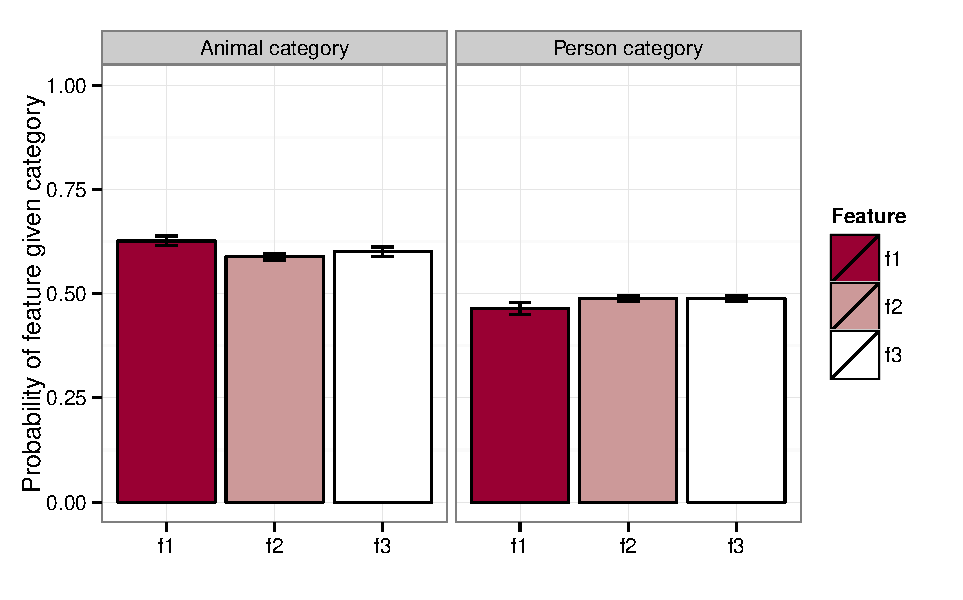
\includegraphics{Plots/priors_bar.pdf}}
%\end{center}
%\caption{Average marginal prior probability ratings for the three features given an animal category or a person category. Error bars are standard error over the $32$ items.} 
%\label{prior}
%\end{figure}

\subsection{Experiment 2: Metaphor Understanding}
\subsubsection{Materials}
We created $32$ scenarios based on the animal categories and results from Experiment 1. In each scenario, a person (e.g. Bob) is having a conversation with his friend about a person that he recently met. Since we are interested in how the communicative goals set up by context affect metaphor interpretation as well as the effectiveness of metaphorical versus literal utterances, we created four conditions for each scenario by crossing vague/specific goals and literal/metaphorical utterances. In vague goal conditions, Bob's friend asks a vague question about the person Bob recently met: ``What is he like?" In specific goal conditions, Bob's friend targets $f_1$ and asks a specific question about the person: ``Is he $f_1$?," where $f_1$ is the most popular adjective for a given animal category $c_a$. In literal conditions, Bob replies with a literal utterance, either by saying ``He is $f_1$." to the question ``What is he like?" or ``Yes." to the question ``Is he $f_1$?". In Metaphorical conditions, Bob replies with a metaphorical statement, e.g. ``He is a $c_a$." where $c_a$ is an animal category. See Table 2 for examples of each condition.

\begin{figure}[t]
\begin{center}
\scalebox{0.55}{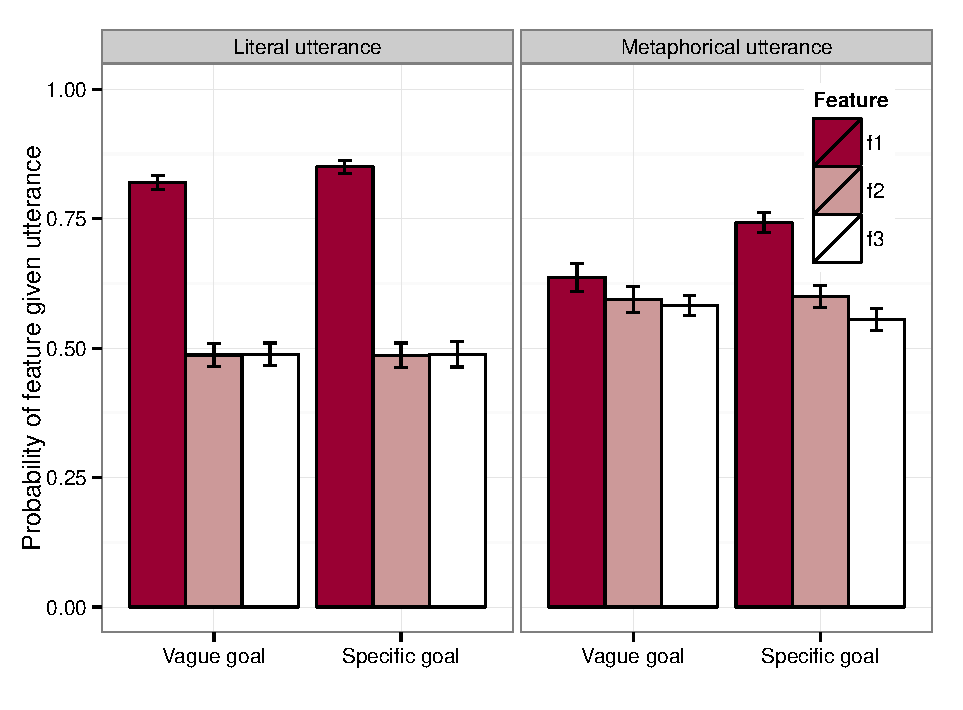
\includegraphics{Plots/human_bar.pdf}}
\end{center}
\caption{Average probability ratings for the three features given a vague/specific goal and a literal/metaphorical utterance. Error bars are standard error over the $32$ items.} 
\label{human_bar}
\end{figure}

\begin{table}[h]
\tabcolsep=0.2cm
\small
\begin{tabular}{llll}
\toprule
Goal & Utterance & Example question & Example utterance \\
\midrule
Vague & Literal & ``What is he like?" & ``He is scary." \\
Specific  & Literal & ``Is he scary?" & ``Yes." \\
Vague & Metaphorical & ``What is he like?" & ``He is a shark." \\
Specific & Metaphorical & ``Is he scary?" & ``He is a shark." \\
\bottomrule
\end{tabular}
\caption{Example scenarios given the four experimental conditions in Experiment 2.s}
\end{table}

\subsubsection{Methods}
$49$ native English speakers with IP addresses in the United States were recruited on Amazon's Mechanical Turk. Each participant completed $32$ trials in random order. The $32$ trials were randomly and evenly assigned to one of the four conditions, i.e. each participant read $8$ scenarios for each condition. For each trial, participants used sliders to indicate the probabilities that the person described has features $f_1$, $f_2$, and $f_3$, respectively.



\subsubsection{Results}
%\begin{figure}[ht]
%\begin{center}
%\scalebox{0.6}{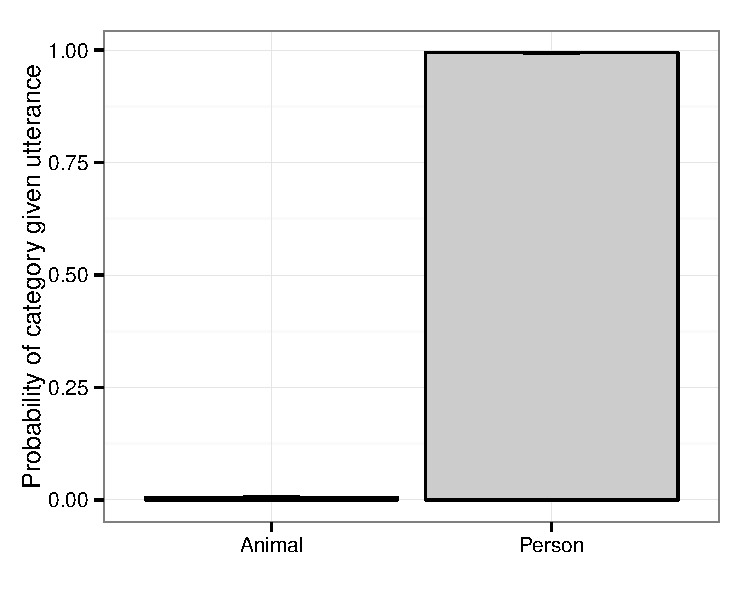
\includegraphics{Plots/model_literal.pdf}}
%\end{center}
%\caption{Model's average marginal category probabilities given a metaphorical utterance ($P(c | u)$). Model's prediction for the animal category is close to $0$ and close to $1$ for the person category. Error bars are standard error over the $32$ items.} 
%\label{scatter_full}
%\end{figure}

For each condition of each scenario, we obtained the average probability ratings for the three features. Figure~\ref{human_bar} shows the average ratings for each feature across animal categories given a vague or specific goal and a literal or metaphorical utterance. When the speaker gives a literal statement directly affirming the presence of $f_1$, participants rate $f_1$ as significantly more likely than when the speaker gives a metaphorical statement ($F(1, 126) = 52.6$, $p < 0.00001$). However, participants rate $f_2$ and $f_3$ as significantly more likely when the speaker produces a metaphorical utterance than when the utterance is literal ($F(1, 126) = 23.7$, $p < 0.0001$; $F(1, 126) =13.66$, $p < 0.0005$). Comparing feature probability ratings in Experiment 2 to the feature priors obtained in Experiment 1b, we can measure how literal and metaphorical utterances change listeners' inferences about a person's features. Given a literal utterance that directly confirms the existence of $f_1$, probability ratings for $f_1$ are significantly higher than the prior probabilities of $f_1$ for a person ($t(63) = 59.19, p < 0.00001$). However, probability ratings for $f_2$ and $f_3$ are not significantly different from their prior probabilities ($t(63) = -0.13, p = 0.89$; $t(63) = 0.03, p = 0.97$). Given a metaphorical utterance, probability ratings for all three features are significantly higher than the prior probabilities ($t(63) = 15.74, p < 0.0001$; $t(63) = 7.29, p < 0.0001$; $t(63) = 5.91, p < 0.0001$). While preliminary, this analysis suggests that metaphorical utterances may convey richer information and update listeners' beliefs along more dimensions than literal utterances.

We now analyze the effect of the speaker's communicative goal on the interpretation of literal or metaphorical utterances. When the speaker's utterance is literal, the probability ratings for $f_1$, $f_2$, and $f_3$ are not significantly different given a vague or a specific question ($(F(1, 62)= 2.73, p =0.1; F(1, 62)=0.0001, p = 0.99; F(1, 62) < 0.0001, p = 0.99$). For metaphorical utterances, however, the question type has an effect on participants' interpretations: participants rate the probability of $f_1$ as significantly higher when the question is specifically about $f_1$ than when it is vague ($F(1, 62) = 10.16$, $p < 0.005$). The probabilities of $f_2$ and $f_3$ are not significantly different given a vague question or a specific question about $f_1$ ($F(1, 62) = 0.04$, $p > 0.05$; $F(1, 62) = 0.8285$, $p > 0.05$). This suggests that people's interpretation of metaphor may be more sensitive to the communicative goals set up by context than their interpretation of literal utterances.

\section{Model Evaluation}
We used the feature priors obtained in Experiment 1b to compute model interpretations of the $32$ metaphors. As discussed in the previous section, the behavioral results in Experiment 2 show evidence that the context set up by a question changes participants' interpretation of a metaphor. Our model naturally accounts for this using the speaker's prior over communicative goals $P(g)$. When a speaker is responding to a vague question, we set the prior distribution for $P(g)$ as uniform. When the speaker is responding to a question specifically about $f_1$, we assume that $P(g_1) > 0.5$ and equal between $P(g_2) = P(g_3)$. Fitting the goal prior parameter to data yields a prior of $P(g_1) = 0.6$ when responding to a specific question about $f_1$. We fit the category prior $P(c_a) = 0.01$ and the speaker optimality parameter $\lambda = 3$. %note that saying "g_1" is a slight abuse of notation given the model definitions above. 

Using these parameters, we obtained interpretation probabilities for each of the $32$ metaphors under both vague and specific goal conditions. For each metaphor and goal condition, the model produces a joint posterior distribution $P(c, \vec f | u)$. We first show a basic but important qualitative result, which is that the model is able to interpret utterances metaphorically. Marginalized over values of $\vec f$, the probability of the person category given the utterance is close to one ($P(c_p | u) = 0.994$), indicating that the pragmatic listener successfully infers that the person described as an animal is actually a person and not an animal. This shows that the model is able to combine prior knowledge and reason about the speaker's communicative goal to arrive at nonliteral interpretations of utterances.

%\begin{figure}[t]
%\begin{center}
%\scalebox{0.6}{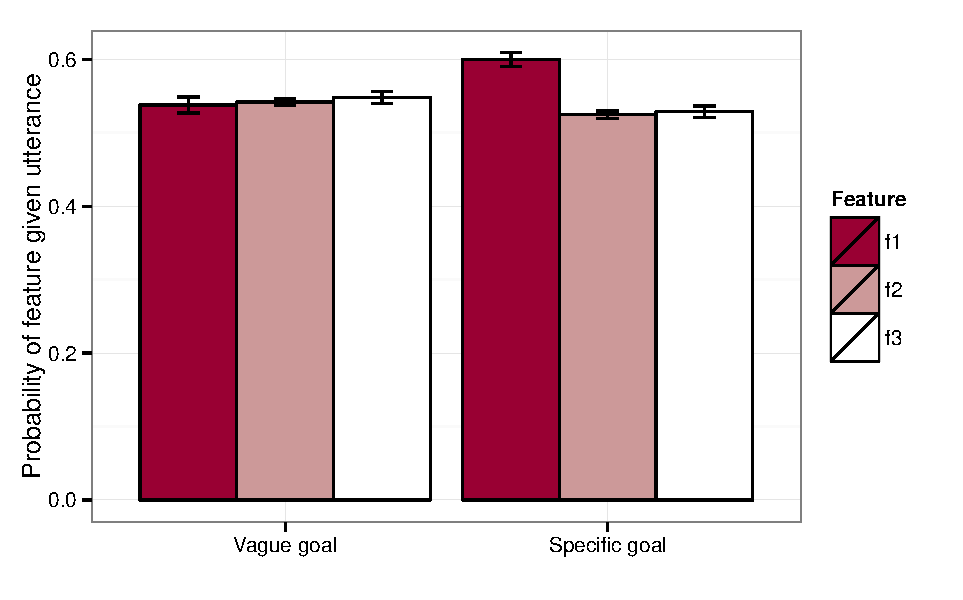
\includegraphics{Plots/model_bar.pdf}}
%\end{center}
%\caption{Model's average } 
%\label{scatter_full}
%\end{figure}

\begin{figure}[t]
\begin{center}
\scalebox{0.6}{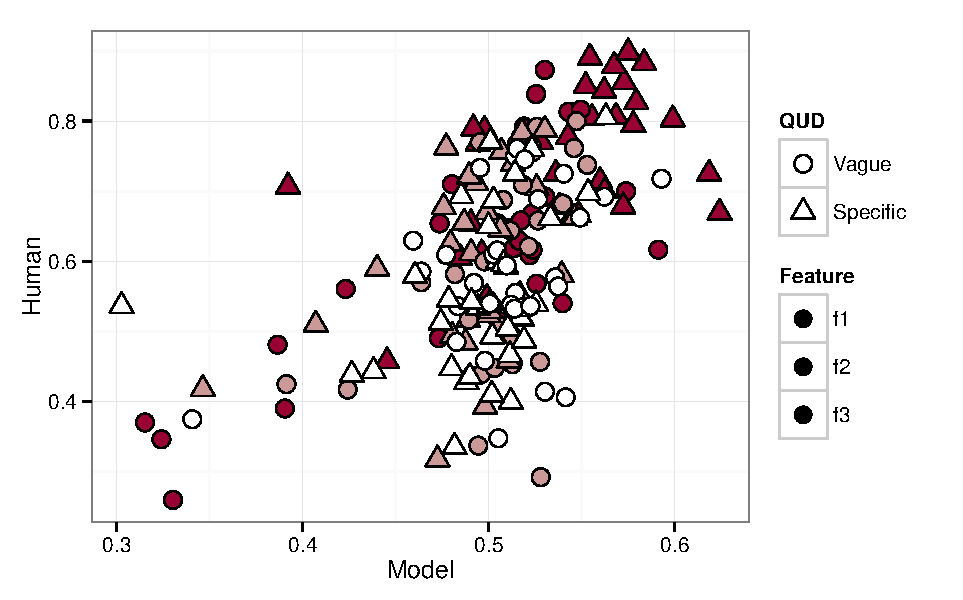
\includegraphics{Plots/scatter_full.pdf}}
\end{center}
\caption{Model predictions ($x$ axis) vs participants' probability ratings ($y$ axis) for $192$ items ($32$ metaphors $\times$ $3$ features $\times$ $2$ goal conditions). Shape of points indicates goal condition and color indicates feature number.} 
\label{scatter_full}
\end{figure}

We now turn to the second component of the interpretation, $P(\vec f | u)$. 
%Figure X shows the average marginal feature probabilities given a vague or specific goal. The model's interpretations are shaped by the communicative goal set up by context, where $f_1$ receives significantly higher marginal probabilities when the speaker is responding to a specific question about $f_1$ ($F(1, 62) =17.92$, $p<0.0001$). This qualitatively matches behavioral results in Figure X. 
To quantitatively evaluate the model's performance, we correlated model predictions with human interpretations of the metaphorical utterances. Given a metaphorical utterance and a vague or specific goal condition, we computed the model's marginal posterior probabilities for $f_1$, $f_2$, and $f_3$. We then correlate these posterior probabilities with participants' probability ratings from Experiment 2. Figure~\ref{scatter_full} plots model interpretations for all metaphors, features, and goal conditions against human judgments. Correlation across the $192$ items ($32$ metaphors $\times$ $3$ features $\times$ $2$ goal conditions) is $0.6$ ($p < 0.001$). The predicted reliability of participants' ratings using the Spearman-Brown prediction formula is $0.828$ ($95\%$ CI $=[0.827, 0.829]$), suggesting first that people do not agree perfectly on metaphorical interpretations, and second that our model captures a significant amount of the reliable variance in the behavioral data. In particular, our model does especially well at predicting participants' judgments of $f_1$, which are the most salient features of the animal categories and were targeted by specific questions in Experiment 2. Correlation between model predictions and human judgments for $f_1$ is $0.7$ ($p < 0.0001$), while the predicted reliability of participants' ratings for $f_1$ is $0.82$ ($95\%$ CI $=[0.818, 0.823]$). 

We now compare our model's performance to a baseline model that also considers the feature priors and the conversational context. We constructed a linear regression model that takes the marginal feature priors for the animal category, the marginal feature priors for the person category, and the vague or specific goal as predictors of participants' ratings. With four parameters, this model produced a fit of $r= 0.45$, which is significantly worse than our model ($p < 0.0001$ on a Cox test). This suggests that our computational model adequately combines people's prior knowledge as well as principles of pragmatics to produce metaphorical interpretations that closely fit behavioral data.

While our model predictions provide a close fit to behavioral data, some residual variance can be further addressed. Previous work has shown that alternative utterances---what the speaker could have said---can strongly affect listeners' interpretation of what the speaker \emph{did} say \cite{bergen2012s}. Our model currently does not take into account the range of alternative utterances (both literal and metaphorical) that a listener considers when interpreting a speaker's utterance. We posit that this may account for some of the variance in the data that our model does not capture. Consider the metaphor ``He is an ant" and the corresponding features \emph{small, strong}, and \emph{busy}. Our model currently assigns a high probability to the feature \emph{strong} given the metaphor, while participants assign it a lower probability. Indeed, this data point has the highest residual in our model fit. To demonstrate that alternative utterances may account for this discrepancy, we construct a model that has ``He is an ox" as an alternative utterance. ``Ox" has features that roughly align with the features of ``ant": \emph{strong, big}, and \emph{slow}. Since \emph{strong} is a higher probability feature for ``ox" than for ``ant," the listener reasons that if the speaker had intended to communicate the feature \emph{strong}, she would have said ``He is an ox" since it optimally satisfies that goal. Since the speaker did \emph{not} produce the utterance ``He is an ox," the listener infers that \emph{strong} is a less probable feature. Adding this alternative utterance to the model indeed lowers the marginal posterior probability of \emph{strong} given the utterance ``He is an ant." As a result, we posit that adding alternative utterances across all animal categories may significantly improve model performance. Constructing a complete set of alternative utterances using our current set of metaphors is not possible because feature combinations are not aligned across animal categories (i.e., different animal categories have different feature sets, and not all features are shared by multiple animals). We aim to address the role of alternative utterances more specifically in future work.

\section{Discussion}
We have presented a computational model that predicts rich metaphorical interpretations using general communicative principles. Besides going beyond the literal meaning of an utterance to infer non-literal interpretations (e.g., John is a person and not a shark), our model provides quantitative judgments about the person's features (e.g., John is very likely scary, dangerous, and mean). Furthermore, behavioral results show that the interpretation of a metaphor is shaped in part by the conversational context, which our model naturally accounts for using communicative goals. Together these results suggest that basic principles of communication may be an important driver of metaphor understanding.

Our model captures several intuitions about communication, including the importance of common ground between listener and speaker, the context-dependence of communicative goals, and the idea that speakers choose to produce utterances that maximize informativeness about features relevant to their communicative goal. Each of these components inspire research questions that can be further investigated using both our modeling framework and experimental paradigm. For example, are listeners less likely to interpret an utterance metaphorically when there is little common ground between speaker and listener? What additional communicative goals are metaphors able to satisfy more effectively than literal utterances? We aim to address these questions in future research to further clarify how communication principles interact to produce metaphorical meaning. We believe that our computational framework advances understanding of the computational basis of metaphor and of communication more generally, and we hope that it will continue to shed metaphorical light on related questions.

%\section{Acknowledgments}
%Place acknowledgments (including funding information) in a section at the end of the paper.



\bibliographystyle{apacite}

\setlength{\bibleftmargin}{.125in}
\setlength{\bibindent}{-\bibleftmargin}

\bibliography{metaphor}


\end{document}
